\documentclass[12pt]{article}
\usepackage{graphicx}
\usepackage[none]{hyphenat}
\usepackage{graphicx}
\usepackage{listings}
\usepackage[english]{babel}
\usepackage{graphicx}
\usepackage{caption} 
\usepackage{booktabs}
\usepackage{array}
\usepackage{amssymb} % for \because
\usepackage{amsmath}   % for having text in math mode
\usepackage{extarrows} % for Row operations arrows
\usepackage{listings}
\lstset{
  frame=single,
  breaklines=true
}
\usepackage{hyperref}
  
%Following 2 lines were added to remove the blank page at the beginning
\usepackage{atbegshi}% http://ctan.org/pkg/atbegshi
\AtBeginDocument{\AtBeginShipoutNext{\AtBeginShipoutDiscard}}


%New macro definitions
\newcommand{\mydet}[1]{\ensuremath{\begin{vmatrix}#1\end{vmatrix}}}
\providecommand{\brak}[1]{\ensuremath{\left(#1\right)}}
\newcommand{\solution}{\noindent \textbf{Solution: }}
\newcommand{\myvec}[1]{\ensuremath{\begin{pmatrix}#1\end{pmatrix}}}
\let\vec\mathbf

\providecommand{\norm}[1]{\left\lVert#1\right\rVert}
\providecommand{\abs}[1]{\left\vert#1\right\vert}
\let\vec\mathbf

\begin{document}

\begin{center}
\title{\textbf{Circles}}
\date{\vspace{-5ex}} %Not to print date automatically
\maketitle
\end{center}
\setcounter{page}{1}

\section{11$^{th}$ Maths - Chapter 10}
This is Problem-3 from Exercise 10.4
\begin{enumerate}
\item Find the centre of a circle passing though the points $(6,-6), (3,-7)$ and $(3,3)$. \\ 
\solution 
The equation of the crcle is given by 
\begin{align}
	\label{eq:circEq1}
	\norm{\vec{x}}^2+2\vec{x}^\top\vec{u}+f = 0 
\end{align}
where
\begin{align}
	\vec{u} = -\vec{c} \text{ and } \\
        \label{eq:fRelation}
	f = \norm{\vec{c}}^2 - r^2
\end{align}
Given points are 
\begin{align}
	\label{eq:circPoints}
     \vec{x_1} = \myvec{6 \\ -6} , \vec{x_2} = \myvec{3 \\-7}, \vec{x_3}= \myvec{3 \\ 3}
\end{align}
Substituting points from \eqref{eq:circPoints} into \eqref{eq:circEq1}
\begin{align}
	\brak{6^2 + \brak{-6}^2}+2\myvec{6 & -6}\vec{u}+f = 0 \\ 
	\implies 2\myvec{6 & -6}\vec{u} + f = -72 \\ 
	\brak{3^2 + \brak{-7}^2}+2\myvec{3 & -7}\vec{u}+f = 0 \\ 
	\implies 2\myvec{3 & -7}\vec{u} + f = -58 \\
	\brak{3^2 + 3^2}+2\myvec{3 & 3}\vec{u}+f = 0 \\ 
	\implies 2\myvec{3 & 3}\vec{u} + f = -18 
\end{align}
Representing the above system of equations in matrix form
\begin{align}
 \myvec{6 & -14 & 1 \\
	12 & -12 & 1 \\
	6 & 6 & 1
	} \myvec {\vec{u} \\
	           f 
		}  = \myvec{-58 \\ -72 \\ -18 }
\end{align}

The augmented matrix is expressed as
\begin{align}
	\myvec{6 & -14 & 1 & \vrule & -58 \\ 
	      12 & -12 & 1 & \vrule & -72 \\
	       6 &  6  & 1 & \vrule & -18 
	     }  
\end{align}
Performing sequence of row operations to transform into an Echelon form
\begin{align}
	\xleftrightarrow[]{{R_2\rightarrow R_2-2R_1}}  
	\myvec{6 & -14 & 1 & \vrule & -58 \\ 
	       0 &  16 & -1 & \vrule & 44 \\
	       6 &  6  & 1 & \vrule & -18 
	     }  \\ 
	\xleftrightarrow[]{{R_3\rightarrow R_3-R_1}}  
	\myvec{6 & -14 & 1 & \vrule & -58 \\ 
	       0 &  16 & -1 & \vrule & 44 \\
	       0 &  20  & 0 & \vrule & 40 
	     }  
\end{align}
\begin{align}
	\xleftrightarrow[]{{R_3\rightarrow R_3-\frac{20}{16}R_2}}  
	\myvec{6 & -14 & 1 & \vrule & -58 \\ 
	       0 &  16 & -1 & \vrule & 44 \\
	       0 &  0  &  \frac{20}{16} & \vrule & -15 
	     }  \\ 
	\xleftrightarrow[R_2\rightarrow \frac{1}{16}R_2 \text{,} R_3\rightarrow \frac{16}{20}R_3]{{R_1\rightarrow \frac{1}{6}R_1}}  
	\myvec{1 & -\frac{14}{6} & \frac{1}{6} & \vrule & -\frac{58}{6} \\ 
	       0 &  1 & -\frac{1}{16} & \vrule & \frac{44}{16} \\
	       0 &  0  &  1  & \vrule & -12 
	     }   
\end{align}
\begin{align}
	\xleftrightarrow[R_2\rightarrow R_2+\frac{1}{16}R_3]{{R_1\rightarrow R_1-\frac{1}{6}R_3}}  
	\myvec{1 & -\frac{14}{6} & 0 & \vrule & -\frac{46}{6} \\ 
	       0 &  1 & 0 & \vrule & 2 \\
	       0 &  0  &  1  & \vrule & -12 
	     }  \\ 
	\label{eq:Solution}
	\xleftrightarrow[]{{R_1\rightarrow R_1+\frac{14}{6}R_2}}  
	\myvec{1 &  0 & 0 & \vrule & -3\\ 
	       0 &  1 & 0 & \vrule & 2 \\
	       0 &  0 & 1 & \vrule & -12 
	     }  \\ 
	\text{So, from } \eqref{eq:Solution} \\
	\vec{u} = \myvec{-3 \\ 2} \\ 
	f = -12 
\end{align}
Since $\vec{u} = -\vec{c}$ , 
\begin{align}
	\vec{c} &= \myvec{ 3 \\ -2} \\
	\eqref{eq:fRelation} \implies r^2 &= \brak{3^2 + \brak{-2}^2} + 12 \\
	 r &= 5
\end{align}
Therefore, the equation of the circle is 
\begin{align}
	\norm{\vec{x}}^2 + 2\myvec{-3 & 2}\vec{x} - 12 = 0 
\end{align}
The relevant diagram is shown in Figure \ref{fig:Fig1}
\begin{figure}[!h]
	\begin{center}
		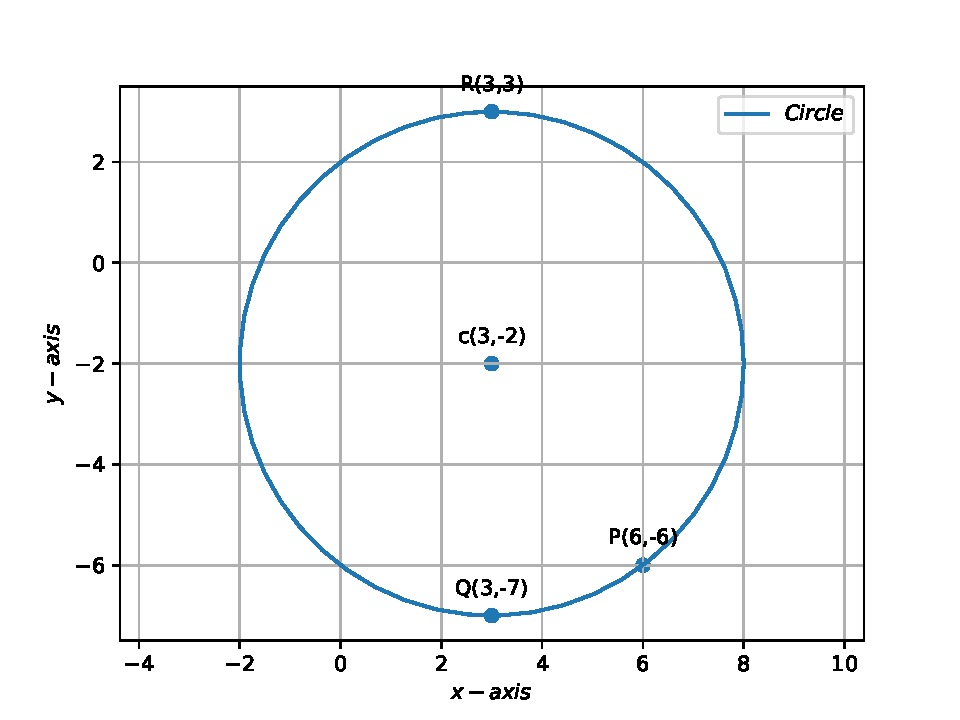
\includegraphics[width=\columnwidth]{./figs/problem3.pdf}
	\end{center}
\caption{}
\label{fig:Fig1}
\end{figure}
\end{enumerate}
\end{document}
